\chapter{Simulateur}
\section{Introduction}
La recherche en data science nécessite souvent l'estimation des densités de probabilités des données utilisés. Dans ce chapitre, nous présentons une application développée dans le but de permettre aux chercheurs d'estimer facilement les densités de probabilités à l'aide d'une interface graphique conviviale.

Notre application se compose de deux sections principales. Dans la première section, les utilisateurs peuvent importer leurs données, telles que des taux de précision, des taux d'erreur, etc., qui vont être considérées comme des variables aléatoires. L'application est ensuite en mesure d'estimer la densité de ces variables en les affichant graphiquement. Pour cette estimation, nous utilisons la méthode du noyau avec l'optimisateur de paramètre de lissage plug-in.

La deuxième section de l'application permet aux utilisateurs de mener des simulations de mélange de trois lois : normale, exponentielle ou uniforme, avec leurs paramètres respectifs. Ensuite, ils peuvent visualiser les densités estimées pour ces distributions en utilisant la méthode de l’histogramme et la méthode du noyau avec ROT, LSCV ou PLUG-IN pour la sélection du paramètre de lissage. De plus, l'application calcule également la densité réelle et EQM relatives aux différentes approches d'estimation. Cela permet de comparer éventuellement des données avec des modèles usuels.

L'application a été développée en utilisant le framework Angular pour la partie frontale et Flask pour la partie backend. Flask a été choisi car sa simplicité d'implémentation en fait un choix approprié. Angular, en tant qu'application SPA (Single Page Application) facilite la communication entre les composants et le chargement du contenu. De plus, il offre la possibilité d'intégrer des graphiques attrayants en utilisant les canvas pré-définis d'Angular. Ainsi, nous n'avons pas besoin d'appeler des graphiques depuis la bibliothèque Matplotlib. Nous pouvons simplement récupérer les listes des densités estimées à partir du backend Flask après le traitement et le calcul.

Ce chapitre présente donc en détail le développement et les fonctionnalités de cette application, ainsi que les résultats obtenus en utilisant différentes méthodes d'estimation pour diverses distributions.

\section{Technologies Utilisées}
Le développement de notre application s'appuie sur deux technologies clés : Angular pour la partie frontend et Python avec Flask pour la partie backend. Le choix de ces technologies a été motivé par leurs avantages spécifiques, qui ont contribué à la réalisation de notre objectif de créer une interface utilisateur conviviale et efficace pour l'estimation des densités de probabilités.
\subsection{Angular}
Angular est  connu pour être un framework de développement d'applications web monopage (SPA - Single-Page Application). Cela signifie que les applications Angular se chargent une seule fois dans le navigateur et mettent à jour dynamiquement le contenu de la page sans nécessiter de rechargement complet.
\subsubsection{Architecture}
Angular suit un modèle architectural appelé MVVM (Model-View-ViewModel), qui est une variante du MVC (Modèle-Vue-Contrôleur). Le MVVM est une conception architecturale qui sépare la logique métier (modèle), la présentation (vue) et la logique de liaison (ViewModel). Dans le MVVM d'Angular, le modèle représente l'état et la logique métier de l'application. La vue est responsable de l'affichage de l'interface utilisateur et de la réception des entrées de l'utilisateur. Le ViewModel agit comme une couche intermédiaire entre le modèle et la vue, gérant la logique de liaison de données, les événements et les interactions avec la vue.

Bien que le MVVM soit une variation du MVC, il diffère légèrement dans la façon dont les responsabilités sont réparties entre les différents éléments. Le ViewModel est plus étroitement lié à la vue, ce qui facilite la gestion de la liaison de données bidirectionnelle et des événements spécifiques à la vue.
\subsubsection{Pourquoi Angular?}
Angular a été choisi pour la partie frontend en raison de sa nature SPA. Cette architecture permet une expérience utilisateur fluide en chargeant une seule page HTML initiale et en mettant à jour dynamiquement le contenu sans recharger complètement la page. Cela offre une navigation rapide et une communication facile entre les composants de l'application. De plus, Angular offre une riche bibliothèque de composants et de directives pré-définis, ce qui facilite la création d'une interface utilisateur attrayante et interactive surtout qu'on va intégrer des graphiques.

\subsection{Flask}
Flask est un framework web minimaliste et puissant pour le développement d'applications web en Python. Il offre une approche simple et flexible pour la création de sites web et d'APIs, en mettant l'accent sur la modularité et la simplicité du code. Flask permet de créer rapidement des applications web légères et efficaces tout en offrant des fonctionnalités de base pour le routage, le rendu de templates et la gestion des formulaires.

\subsubsection{Architecture}
L'architecture de Flask suit le modèle de développement web appelé "modèle-vue-contrôleur" (MVC), bien que de manière plus légère et flexible par rapport à certains frameworks MVC complets. Flask encourage une structure de code modulaire et permet aux développeurs de choisir les outils et bibliothèques qu'ils préfèrent pour gérer les différentes parties de l'application.

\subsubsection{Pourquoi Flask?}
Flask a été choisi comme framework backend pour sa simplicité d'utilisation, sa légèreté et sa parfaite intégration avec Python. Cette combinaison nous a permis d'adopter une approche centrée sur les contrôleurs et les modèles en renvoyant des réponses JSON plutôt que de générer des vues HTML. Ainsi, nous avons pu concevoir une architecture efficace, tout en offrant une flexibilité aux utilisateurs pour choisir et visualiser les densités estimées pour différentes distributions. En résumé, le choix de Flask et Python nous a permis de développer rapidement une application avec des contrôleurs et des modèles, tout en fournissant des réponses JSON pour une expérience utilisateur fluide et une gestion simplifiée des données.




\section{Présentation de l'application}
\subsection{Description}
L'objectif de notre application est de mettre à la disposition des chercheurs un outil leur permettant d'estimer les densités de probabilités des variables aléatoires. Pour cela, nous utilisons la méthode du noyau avec une optimisation du paramètre de lissage en utilisant la méthode PLUG in. De plus, une partie de l'application vise à comparer les performances des estimateurs pour des lois usuelles.

La première fonctionnalité de l'application permet à l'utilisateur de faire des simulations en choisissant trois distributions (dont une est obligatoire et les deux autres optionnelles). Pour chaque distribution, l'utilisateur peut sélectionner l'une des trois lois disponibles : normale, exponentielle ou uniforme. De plus, il peut spécifier les paramètres de chaque distribution. Cette fonctionnalité donne à l'utilisateur la possibilité de jouer avec la complexité des distributions afin d'étudier plus précisément les performances des estimateurs. Les méthodes qui vont être utilisées dans les estimations sont la méthode du noyau ( ROT, LSCV et Plug-in) et la méthode de l'histogramme.

La deuxième partie de l'application permet à l'utilisateur de télécharger des fichiers texte contenant des valeurs, qui peuvent être des taux de précision d'un classifieur, par exemple, comme nous l'avons fait dans le chapitre précédent. Ensuite, la densité de probabilité de ces variables est calculée dans le backend de l'application et affichée dans un graphique pour l'utilisateur. L'utilisateur a également la possibilité de télécharger plusieurs fichiers et de travailler avec plusieurs variables, ce qui lui permet de visualiser les densités de ces variables sur le même graphique et de déterminer le meilleur classifieur, comme nous l'avons fait dans le chapitre précédent.

\subsection{Architecture}
    L'architecture de mon application est représentée dans la figure ci-dessous. Les composants utilisés en Angular et les modules en Flask sont représentés par des rectangles noirs. Les flèches indiquent les interactions entre les différents composants et modules. Les notes en jaune représentent les actions spécifiques réalisées dans chaque partie de l'application.
    
\begin{figure}[!h]
  \centering
  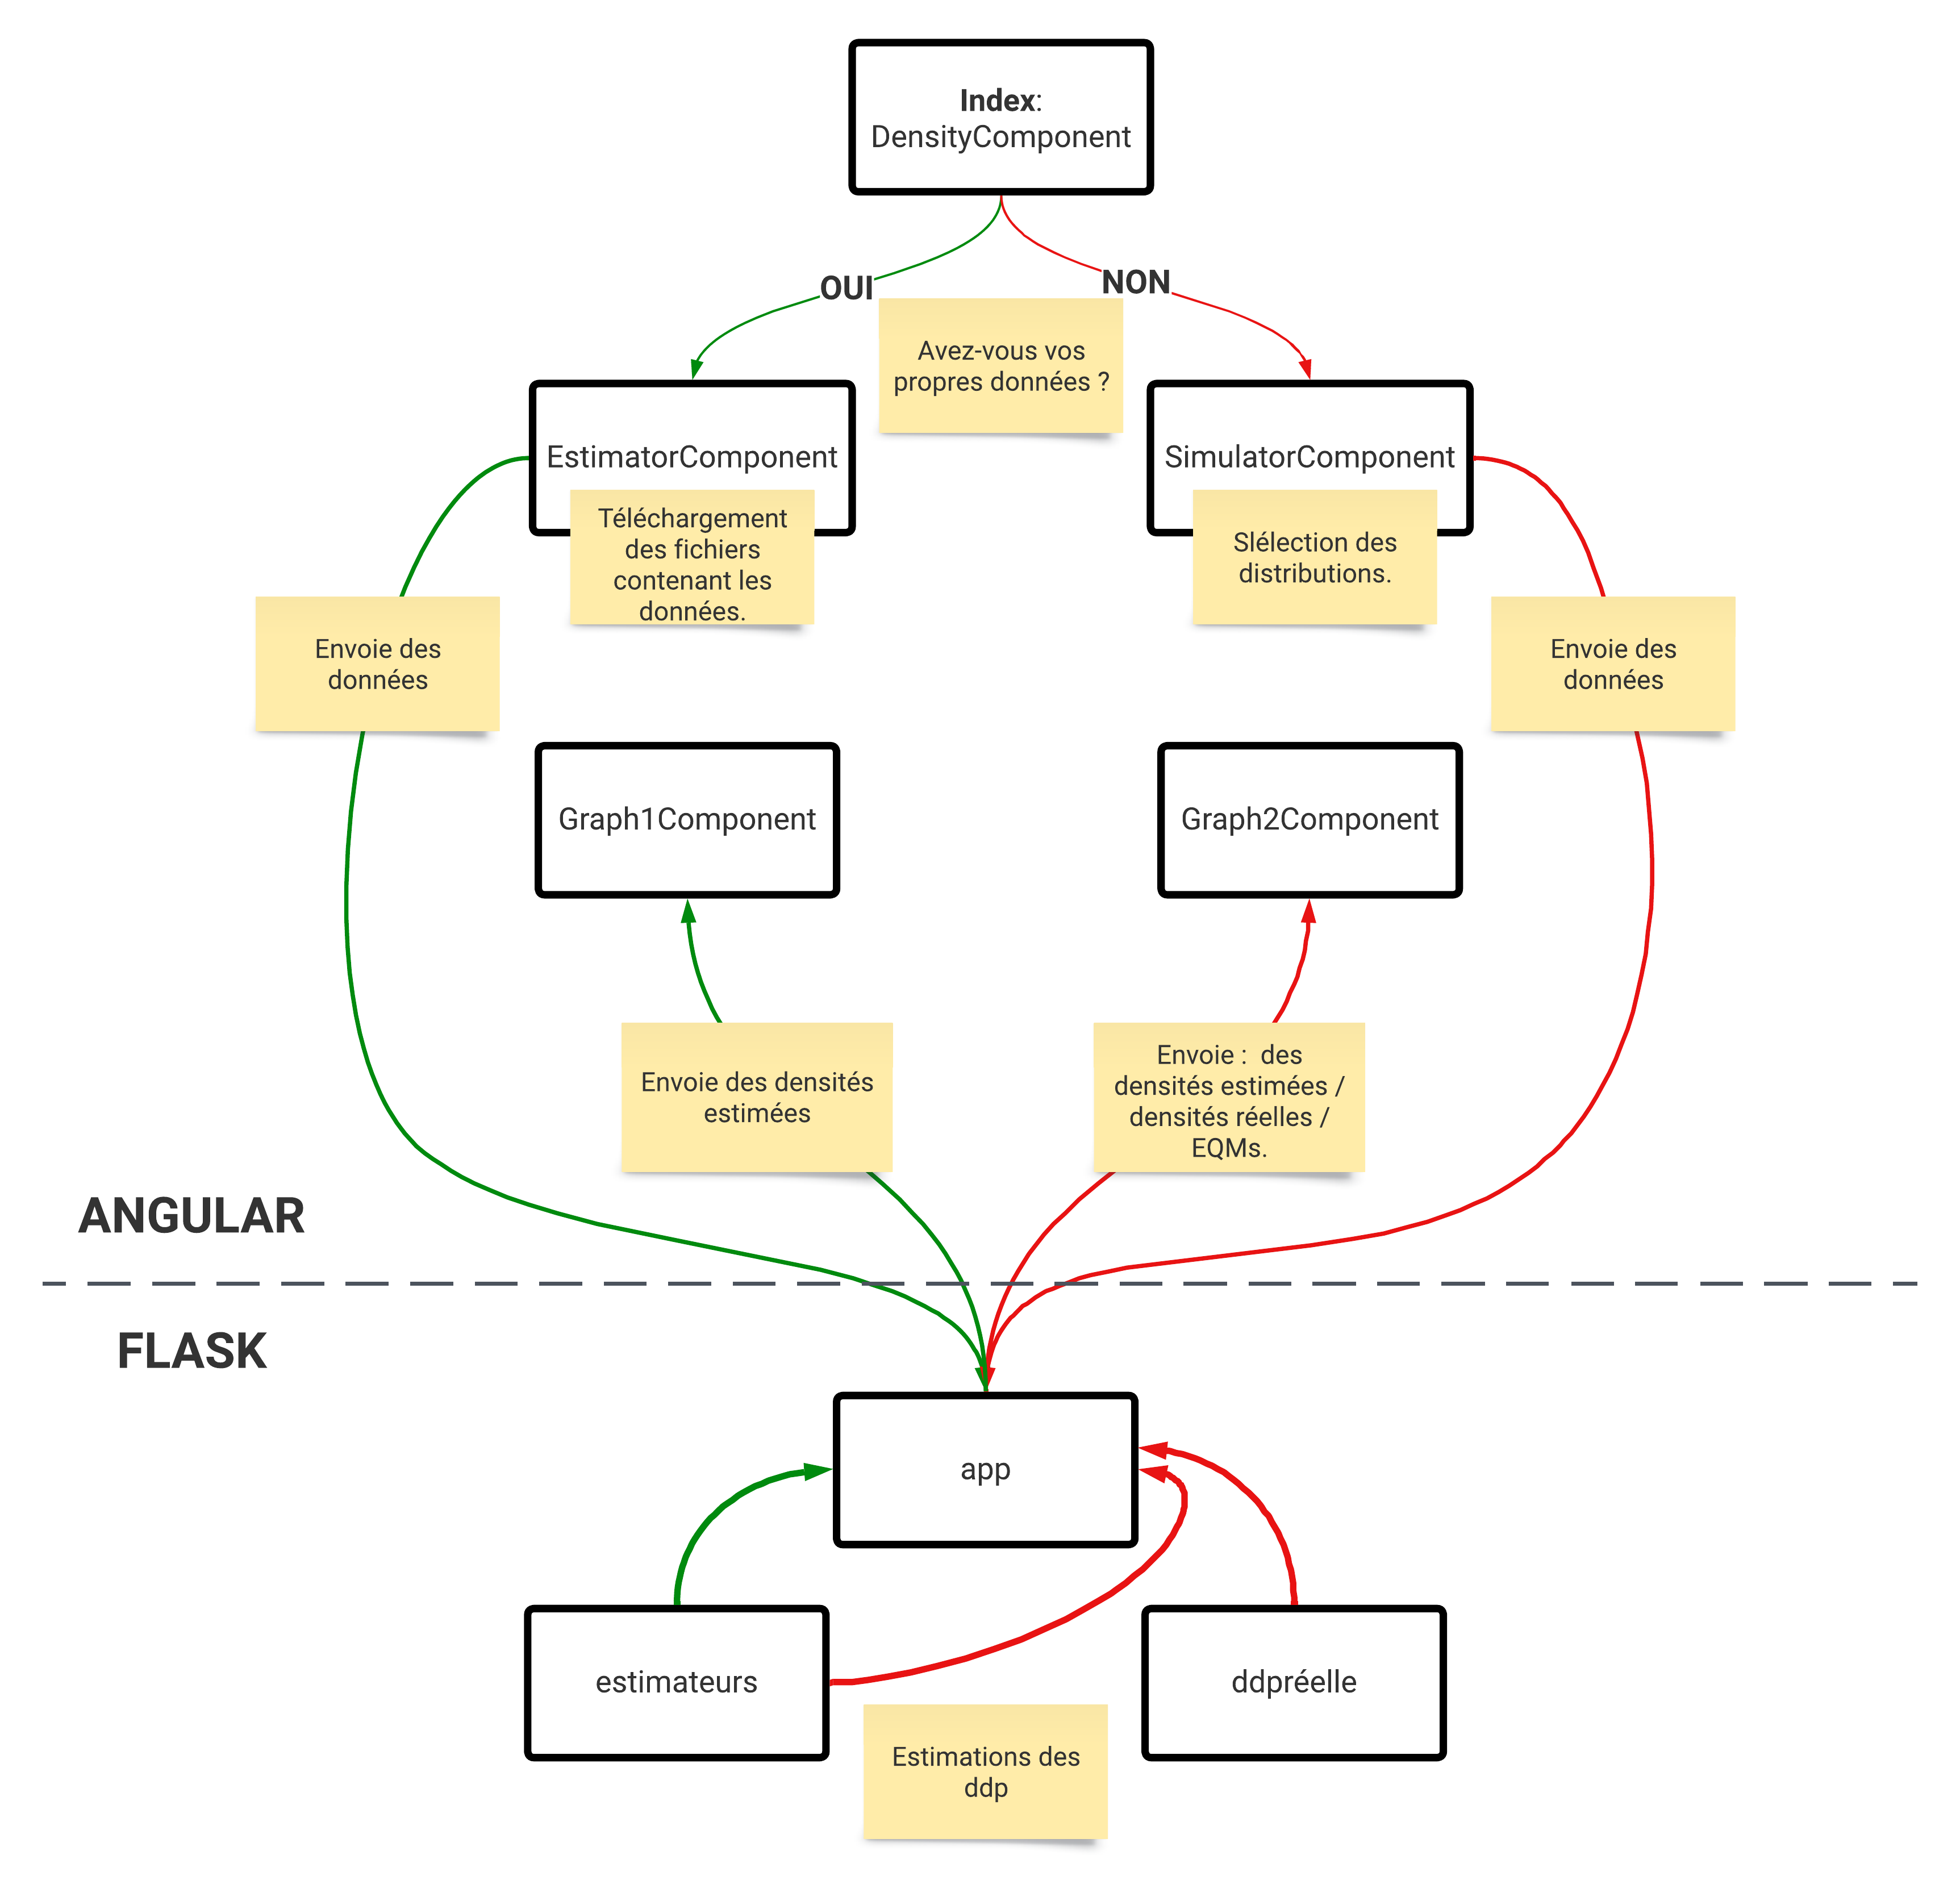
\includegraphics[width=18cm,height=21cm]{Figure 5.1.png}
  \caption{Architecture de l'application}
  \label{fig:Architecture de l'application}
\end{figure}
\clearpage

\section{Guide pratique}
En premier lieu, vous avez la possibilité de choisir entre deux options : importer vos propres données ou effectuer des simulations (voir Figure 5.2). Cette fonctionnalité vous offre une grande flexibilité en vous permettant de travailler avec vos propres données réelles ou de créer des scénarios simulés pour une analyse plus approfondie.

\begin{figure}[!h]
  \centering
  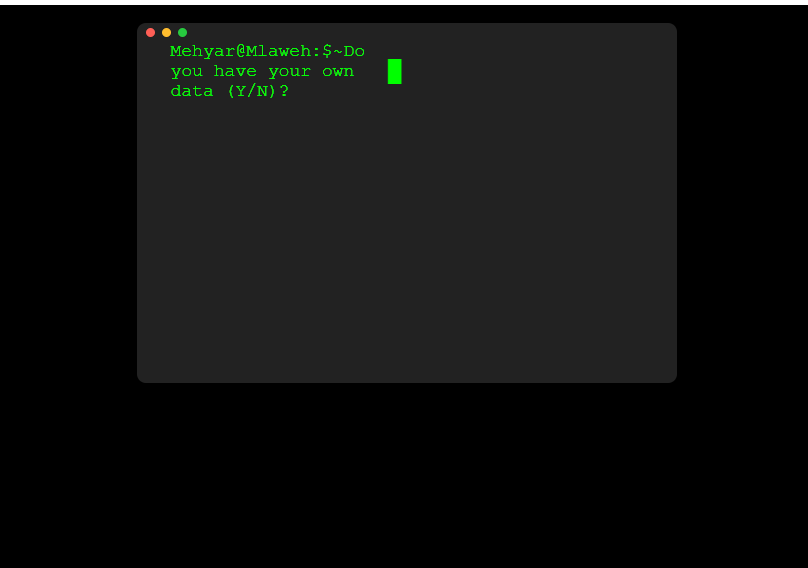
\includegraphics[width=15cm,height=10cm]{Figure 5.2.png}
  \caption{Page Index - Simulateur}
  \label{fig:Architecture de l'application}
\end{figure}

Dans la figure ci-dessous ( Figure 5.3), nous présentons la partie de l'application dédiée à la configuration des distributions à estimer. L'utilisateur a la possibilité de choisir jusqu'à trois distributions pour effectuer l'estimation, tandis que la deuxième et troisième distribution sont facultatives, offrant ainsi une flexibilité pour ajuster la complexité du mélange. Cette fonctionnalité permet à l'utilisateur de personnaliser les paramètres des distributions et d'explorer différents scénarios pour l'estimation. Et dans la figure 5.4, nous pouvons voir la densité réelle du mélange et les densités estimées par la méthode de l'histogramme et la méthode du noyau avec Plug-in , ROT et LSCV. 
\clearpage

\begin{figure}[!h]
  \centering
  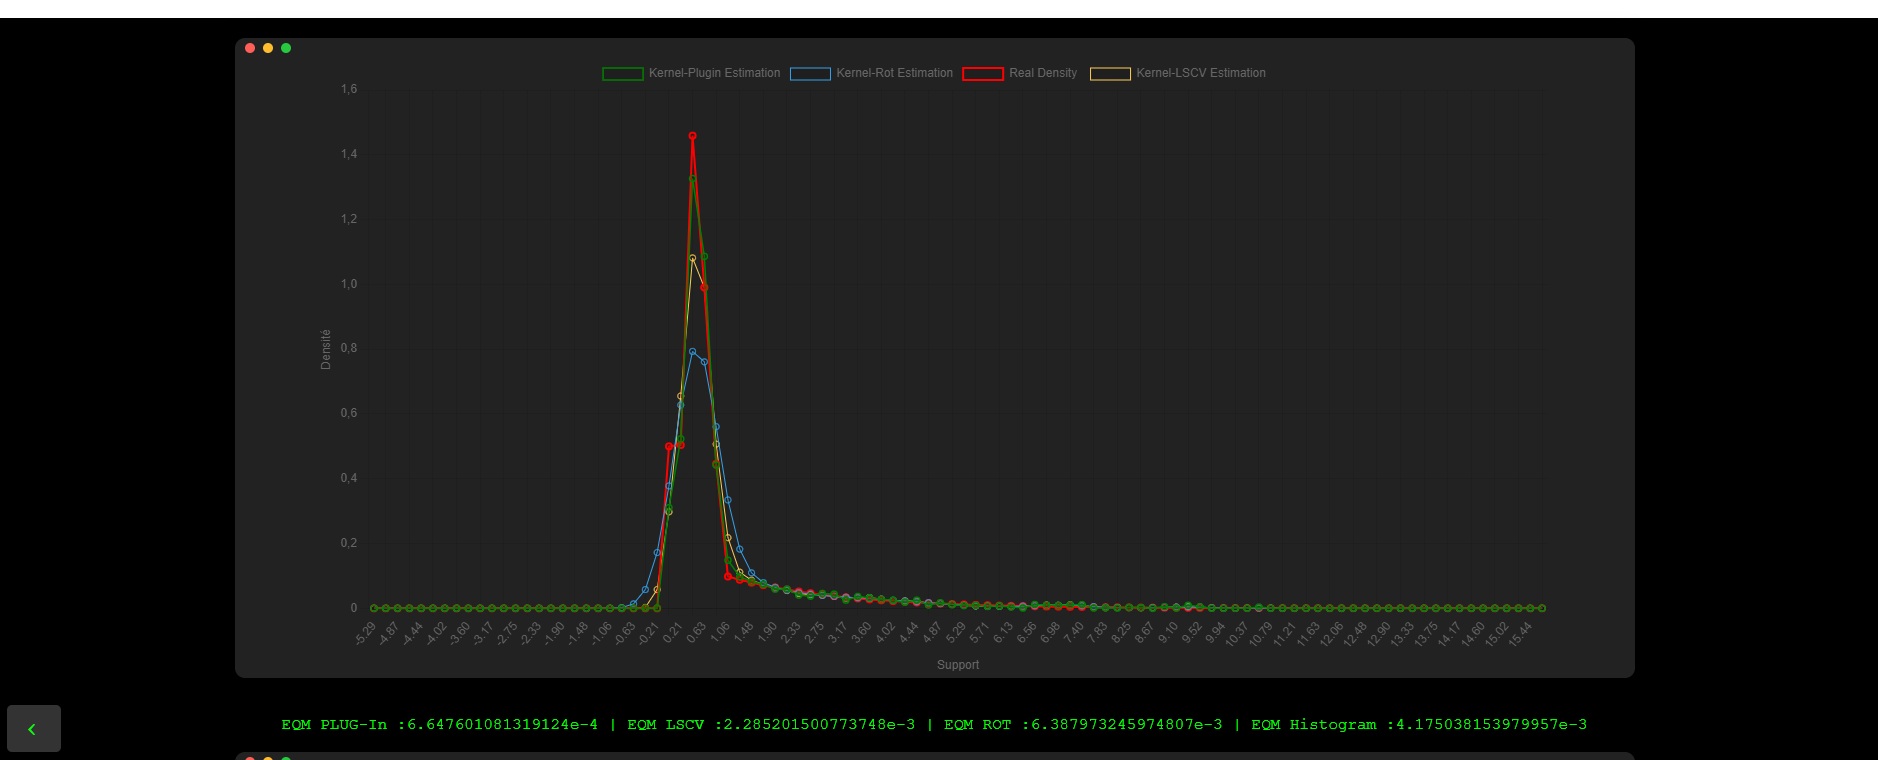
\includegraphics[width=15cm,height=9cm]{Figure 5.3.png}
  \caption{Choix des distributions - Simulateur}
  \label{fig:Architecture de l'application}
\end{figure}
\begin{figure}[!h]
  \centering
  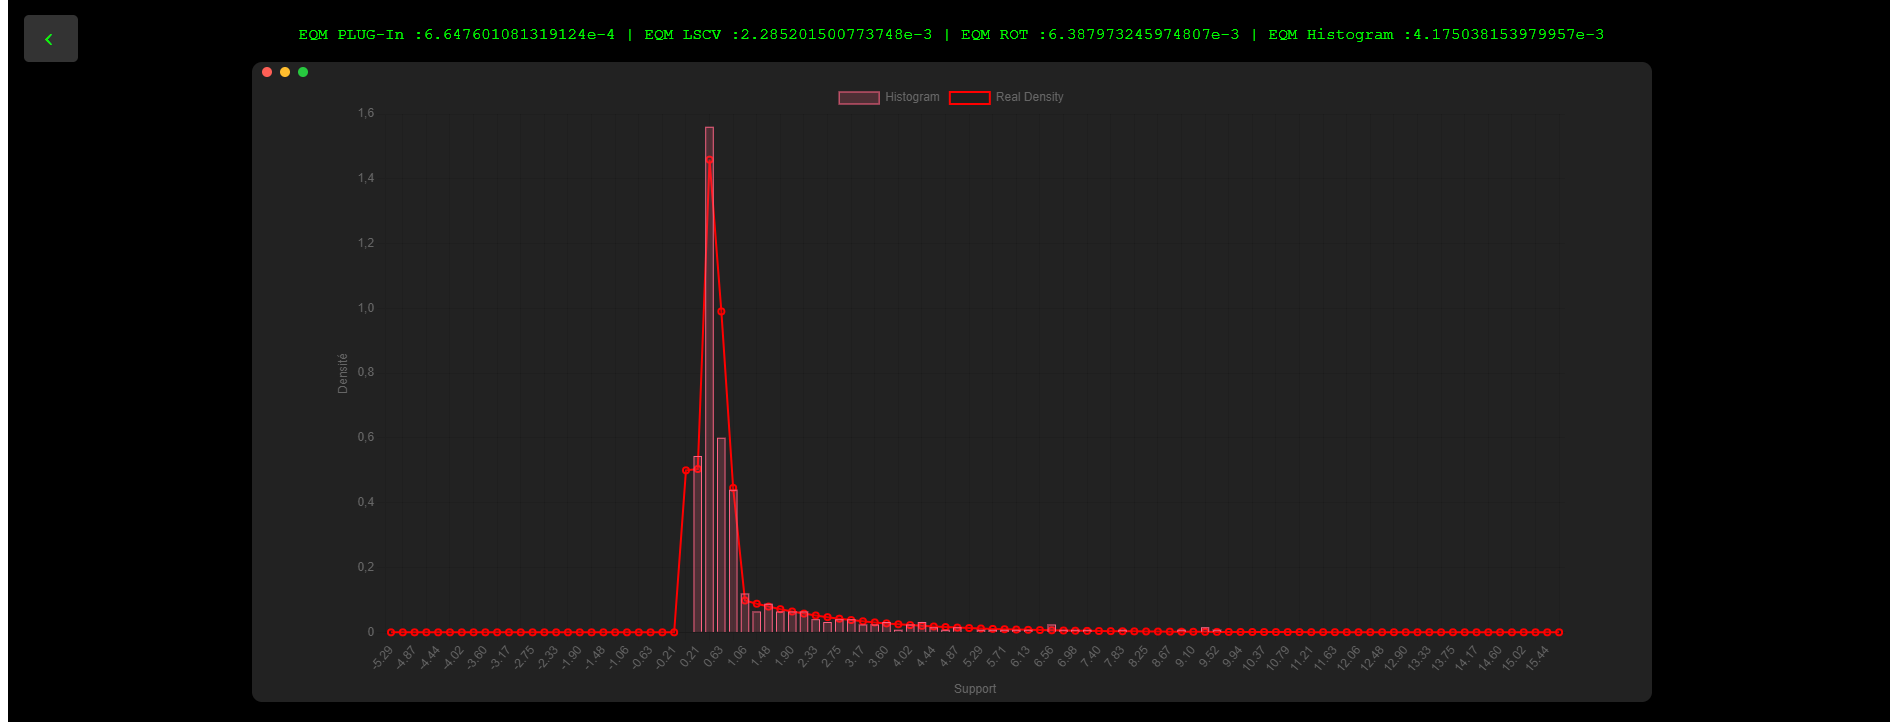
\includegraphics[width=15cm,height=9cm]{Figure 5.4.png}
  \caption{Résultat des simulations - Simulateur}
  \label{fig:Architecture de l'application}
\end{figure}
\clearpage
Si vous choisissez d'importer vos propres données, vous devez sélectionner des fichiers texte (.txt) contenant les données que vous souhaitez estimer leur densité de probabilités( Figure 5.5). Assurez-vous que les données sont séparées par des points-virgules (;) et évitez d'inclure des espaces blancs. Vous avez la possibilité d'importer plusieurs fichiers et de supprimer un fichier importé si nécessaire. Une fois que vous avez importé vos données, il vous suffit de cliquer sur le bouton "Estimer" pour accéder au graphique affichant les densités de probabilités en utilisant la méthode du noyau avec Plug-in pour la sélection du paramètre de lissage.\\
\begin{figure}[!h]
  \centering
  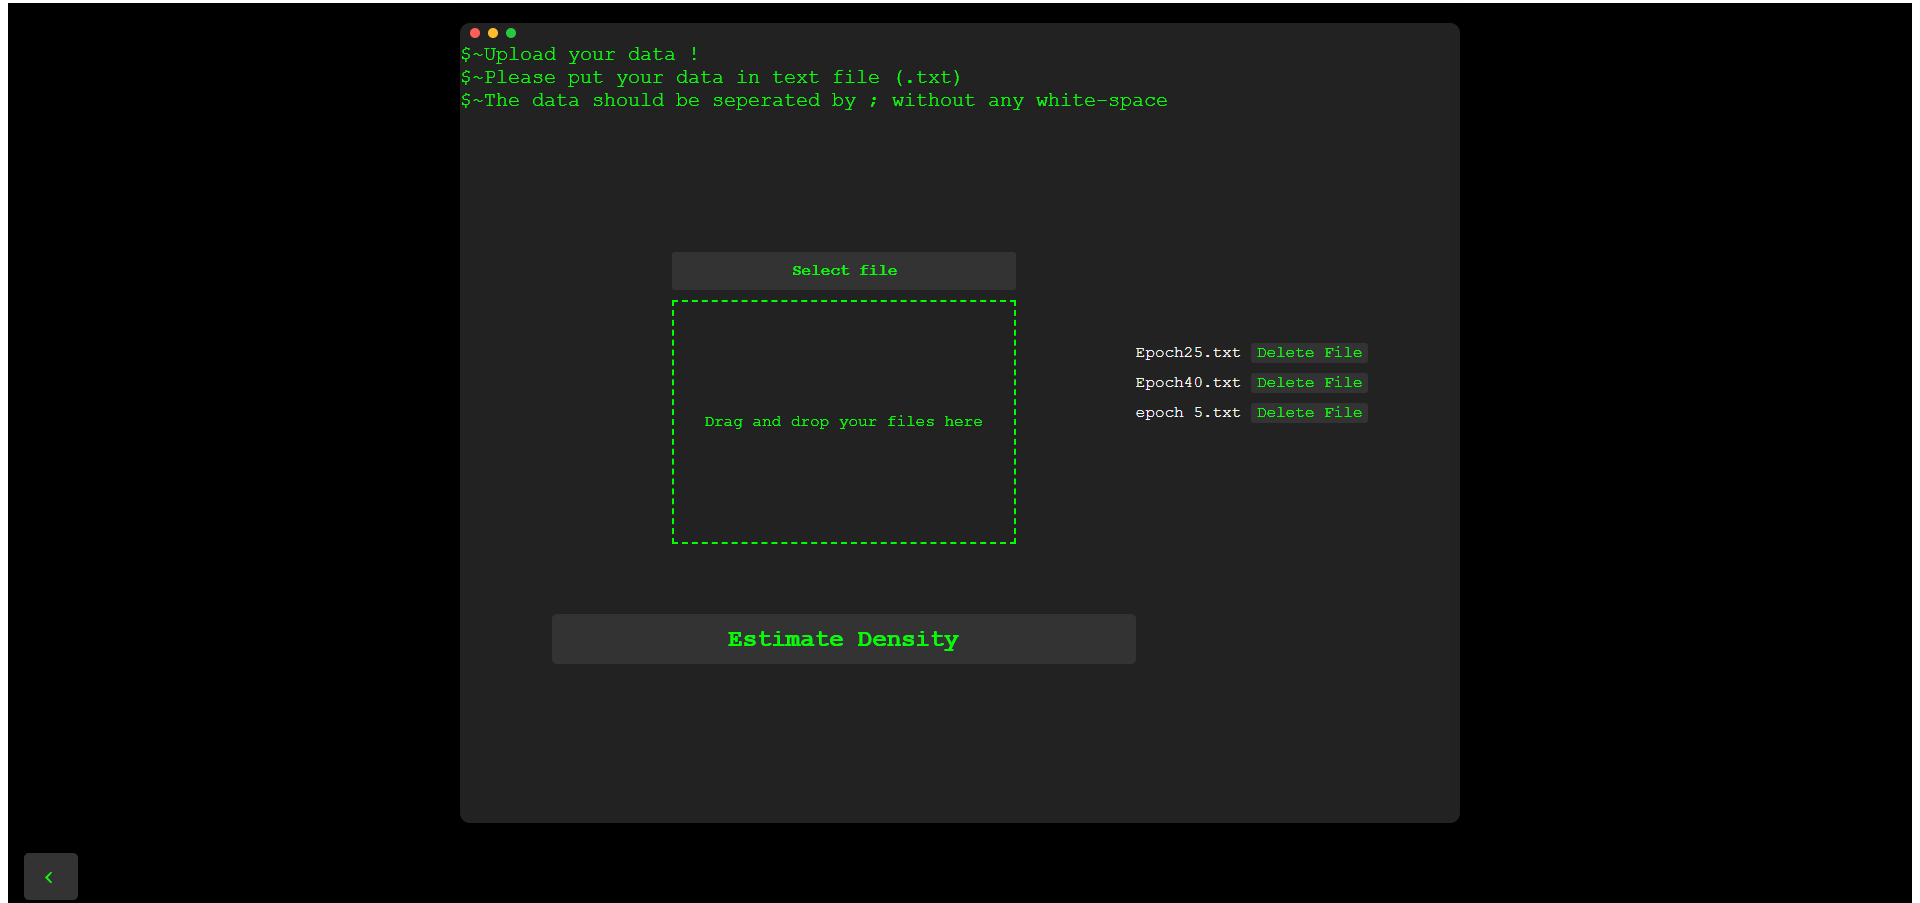
\includegraphics[width=15cm,height=9cm]{Figure 5.5.png}
  \caption{Importation des données - Simulateur}
  \label{fig:Architecture de l'application}
\end{figure}


Dans le graphique ( Figure 5.6), chaque densité de probabilité sera étiquetée avec le nom du fichier correspondant aux données. Toutes les densités seront affichées sur le même graphique, ce qui vous permettra de comparer visuellement les différentes distributions. Vous aurez également la possibilité de cliquer sur l'étiquette de chaque densité pour masquer ou afficher la densité des données d'un fichier spécifique. Cela vous permettra de visualiser sélectivement les densités qui vous intéressent le plus. \\
\begin{figure}[!h]
  \centering
  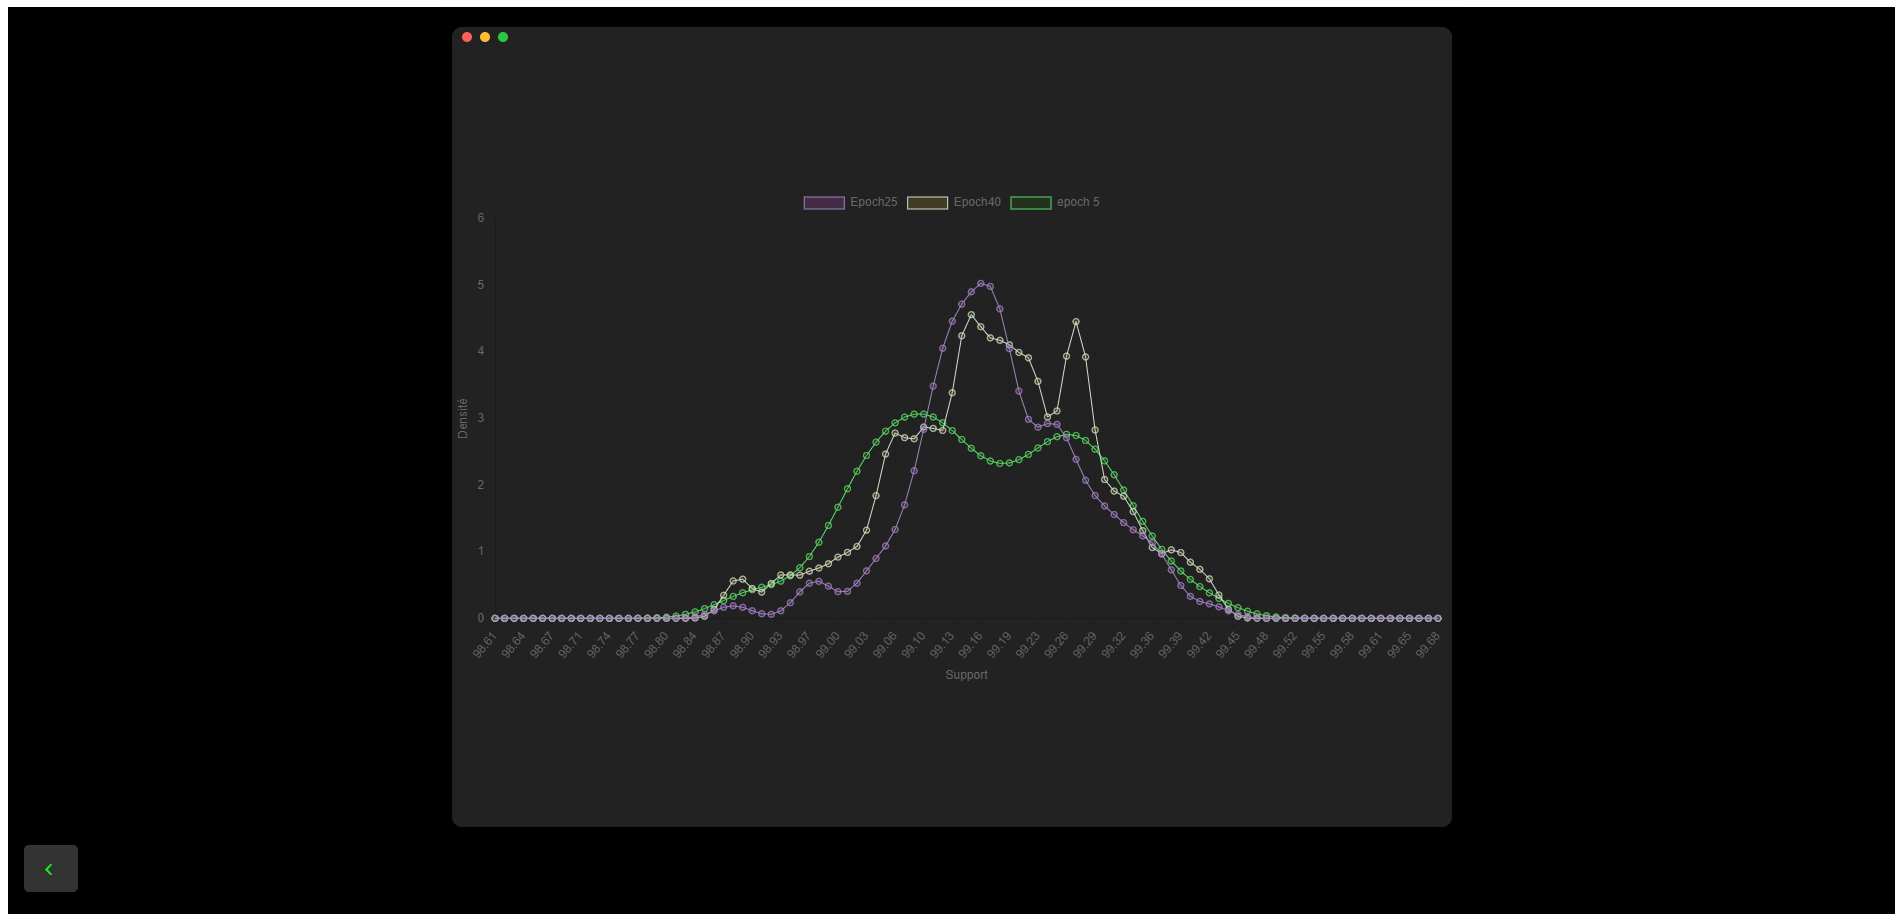
\includegraphics[width=15cm,height=9cm]{Figure 5.6.png}
  \caption{Résultat des estimations - Simulateur}
  \label{fig:Architecture de l'application}
\end{figure}
\newpage
\section{Conclusion}
En conclusion, cette application offre une solution puissante et polyvalente aux chercheurs et informaticiens pour estimer les densités de probabilité des variables aléatoires. Elle constitue un outil essentiel pour comparer les estimateurs et déterminer le meilleur classifieur ou algorithme adapté à leurs besoins.

Pour les chercheurs, cette application leur permet d'explorer et de comparer différents estimateurs, ce qui facilite leur recherche et leur permet de prendre des décisions éclairées en matière d'estimation des densités de probabilité. Ils peuvent ainsi évaluer la performance des estimateurs et identifier celui qui convient le mieux à leur contexte spécifique.

Quant aux informaticiens, cette application leur offre la possibilité d'estimer les densités des variables aléatoires, ce qui leur permet de mieux comprendre et analyser les données. Ils peuvent ainsi prendre des décisions basées sur des informations précises et fiables, notamment dans le cadre du développement de classifieurs et d'algorithmes.

En plus des avantages mentionnés précédemment, cette application offre également des perspectives intéressantes pour son amélioration et son évolution continue. Deux aspects clés peuvent être envisagés pour développer davantage cette application.

Tout d'abord, en ce qui concerne la partie simulation, il est possible d'ajouter d'autres lois de probabilité pour générer des données simulées. Cela élargirait la gamme de distributions disponibles et offrirait une flexibilité supplémentaire pour les expérimentations et les analyses.

Deuxièmement, en ce qui concerne les estimateurs de densité, il serait intéressant de permettre aux utilisateurs de choisir librement les paramètres de lissage pour des estimateurs tels que l'histogramme ou le noyau. Cette fonctionnalité permettrait aux utilisateurs d'explorer et de visualiser l'impact du paramètre de lissage sur les estimations de densité, mettant ainsi en évidence l'influence de ce paramètre sur la précision et la lissage de la courbe estimée.